\documentclass[11pt]{article}

\usepackage[T1]{fontenc}
\usepackage[utf8]{inputenc}
\usepackage{lmodern}
\usepackage[margin=1in]{geometry}
\usepackage{xcolor}
\usepackage{graphicx}
\usepackage{tikz}
\usepackage{booktabs}
\usepackage{longtable}
\usepackage{enumitem}
\usepackage{hyperref}
\usepackage{listings}
\usetikzlibrary{arrows.meta,fit,positioning}

\setlength{\emergencystretch}{2em}

\hypersetup{
  colorlinks=true,
  linkcolor=blue!55!black,
  urlcolor=blue!55!black
}

\lstdefinelanguage{EasyCrypt}{
  morekeywords={
    require,import,theory,end,section,lemma,proof,qed,op,pred,type,module,
    declare,clone,proc,if,then,else,while,return,forall,exists,real,int,bool
  },
  sensitive=true,
  morecomment=[l]{//},
  morecomment=[s]{(*}{*)},
  morestring=[b]"
}

\lstset{
  basicstyle=\ttfamily\small,
  breaklines=true,
  columns=fullflexible,
  frame=single,
  framerule=0.3pt,
  rulecolor=\color{black!30},
  xleftmargin=0.5em,
  xrightmargin=0.5em,
  aboveskip=0.7em,
  belowskip=0.7em
}

\newcommand{\file}[1]{\nolinkurl{#1}}
\newcommand{\ec}[1]{\nolinkurl{#1}}
\newcommand{\eufcma}{EUF-CMA}

\title{Following the HAETAE Machine-Checked Provable-Security Verification}
\author{HAETAE EasyCrypt proof guide}
\date{May 2026}

\begin{document}
\maketitle

\begin{abstract}
This guide explains how to follow the machine-checked provable-security
verification for the HAETAE EasyCrypt development from a fresh checkout of the
project directory.  It tells the reader what is checked, what is deliberately
outside the proof gate, how to run the verifier, how to read the proof files in
a useful order, and how to make changes without silently weakening the checked
surface.
\end{abstract}

\tableofcontents

\section{What This Guide Covers}

The checked artifact is a conditional, game-based EasyCrypt proof for the
formal HAETAE random-oracle signature model.  The central claim is not that all
implementation code, concrete SHAKE security, or lattice assumptions are proved
from first principles.  The checked claim is that the EasyCrypt model's
\eufcma{} advantage is bounded by the concrete loss expression assembled in the
reduction files, assuming the abstract MLWE, Module-SIS, and bimodal
self-target hardness games represented in the model.

The source of truth for the checked proof surface is the manifest:

\begin{lstlisting}[language=bash]
provable-security/proof-files.txt
\end{lstlisting}

Files in \file{rubbish/} are archival material and are not part of the
machine-checked proof gate.  Generated known-answer-test files and older bridge
files may be useful as historical or validation artifacts, but they are not
inputs to the provable-security verification described here.

\section{Starting From a Fresh Terminal}

Begin in the \file{haetae-security} directory.  In this repository snapshot the
directory is:

\begin{lstlisting}[language=bash]
cd /home/hacker-code-j/Desktop/2026/HAETAE/kpqc-sig-haetae-jasmin-easycrypt/haetae-security
\end{lstlisting}

Confirm that EasyCrypt is available:

\begin{lstlisting}[language=bash]
easycrypt --version
\end{lstlisting}

Confirm that the proof gate and manifest are present:

\begin{lstlisting}[language=bash]
test -f provable-security/verify-provable-security.sh
test -f provable-security/proof-files.txt
test -d provable-security/easycrypt
\end{lstlisting}

The verification script uses the \file{easycrypt} executable by default.  To use
a different executable, set the \file{EASYCRYPT} environment variable:

\begin{lstlisting}[language=bash]
EASYCRYPT=/path/to/easycrypt sh provable-security/verify-provable-security.sh
\end{lstlisting}

\section{First Full Verification Run}

Run the proof gate before reading or editing anything:

\begin{lstlisting}[language=bash]
sh provable-security/verify-provable-security.sh
\end{lstlisting}

The script compiles each manifest file from \file{provable-security/easycrypt/}
with this shape of command:

\begin{lstlisting}[language=bash]
easycrypt compile provable-security/easycrypt/<file>.ec \
  -max-provers 1 \
  -I provable-security/easycrypt \
  -I kyber-security
\end{lstlisting}

The run is successful only if the final line is:

\begin{lstlisting}
RESULT: PASS
\end{lstlisting}

Logs are written to:

\begin{lstlisting}[language=bash]
provable-security/logs/
\end{lstlisting}

The most useful summary file is:

\begin{lstlisting}[language=bash]
provable-security/logs/last-run-summary.txt
\end{lstlisting}

If a file fails, inspect the corresponding log first.  For example:

\begin{lstlisting}[language=bash]
sed -n '1,160p' provable-security/logs/HAETAE_Security.log
tail -n 120 provable-security/logs/HAETAE_Security.log
\end{lstlisting}

\section{The Checked Proof Surface}

The current manifest contains exactly sixteen EasyCrypt files:

\begin{longtable}{p{0.34\textwidth}p{0.56\textwidth}}
\toprule
\textbf{File} & \textbf{Role in the checked proof} \\
\midrule
\endfirsthead
\toprule
\textbf{File} & \textbf{Role in the checked proof} \\
\midrule
\endhead
\file{HAETAE_Security.ec} &
Top-level correctness and \eufcma{} theorem composition. \\
\file{Sig_ROM.ec} &
Generic signature games, random-oracle interfaces, and NMA-to-CMA adapter. \\
\file{HAETAE_HopGames.ec} &
Detailed hybrid games, signing simulation, ROM-internal games, sampler
freshness, and budgeted lifting. \\
\file{HAETAE_Reductions.ec} &
Concrete loss terms, query-budget arithmetic, and final bound expressions. \\
\file{HAETAE_ROM.ec} &
HAETAE random-oracle query and output model. \\
\file{HAETAE_ROM_Programming.ec} &
Counted random-oracle programming sites, bad events, and programming bounds. \\
\file{HAETAE_Scheme.ec} &
Instantiation of the generic signature interface with HAETAE procedures. \\
\file{HAETAE_Transcript.ec} &
Transcript records, validity predicates, and extraction-facing lemmas. \\
\file{HAETAE_Events.ec} &
Named rejection, acceptance, and verification event vocabulary. \\
\file{HAETAE_Assumptions.ec} &
Abstract hardness games and reduction interfaces. \\
\file{HAETAE_Distributions.ec} &
Sampling distributions and distributional support facts. \\
\file{HAETAE_Rejection.ec} &
Rejection predicates, rejection-sampling support, and loss accounting. \\
\file{HAETAE_Algebra.ec} &
HAETAE algebraic data types, polynomial operations, and algebraic lemmas. \\
\file{HAETAE_Params.ec} &
Parameter modes and constants. \\
\file{HAETAE_FIPS202.ec} &
Modeled FIPS202/SHAKE support used by the HAETAE model. \\
\file{HAETAE_Keccak1600.ec} &
Keccak state and low-level hash support definitions. \\
\bottomrule
\end{longtable}

The copied files in \file{provable-security/easycrypt/} are the files compiled
by the proof gate.  The project-root copies are kept in sync for ordinary
editing and compatibility with the surrounding repository layout.

\section{Structure Diagram and Design Rationale}

Figure~\ref{fig:ec-file-structure} shows the intended structure of the active
EasyCrypt files.  The arrows point from a file that supplies definitions,
interfaces, games, or lemmas to a file that consumes them.  This is a
proof-architecture diagram, not a claim that every EasyCrypt library import is
drawn; standard-library imports such as \file{AllCore}, \file{List}, and
\file{Distr} are deliberately omitted.

\begin{figure}[p]
\centering
\resizebox{\textwidth}{!}{%
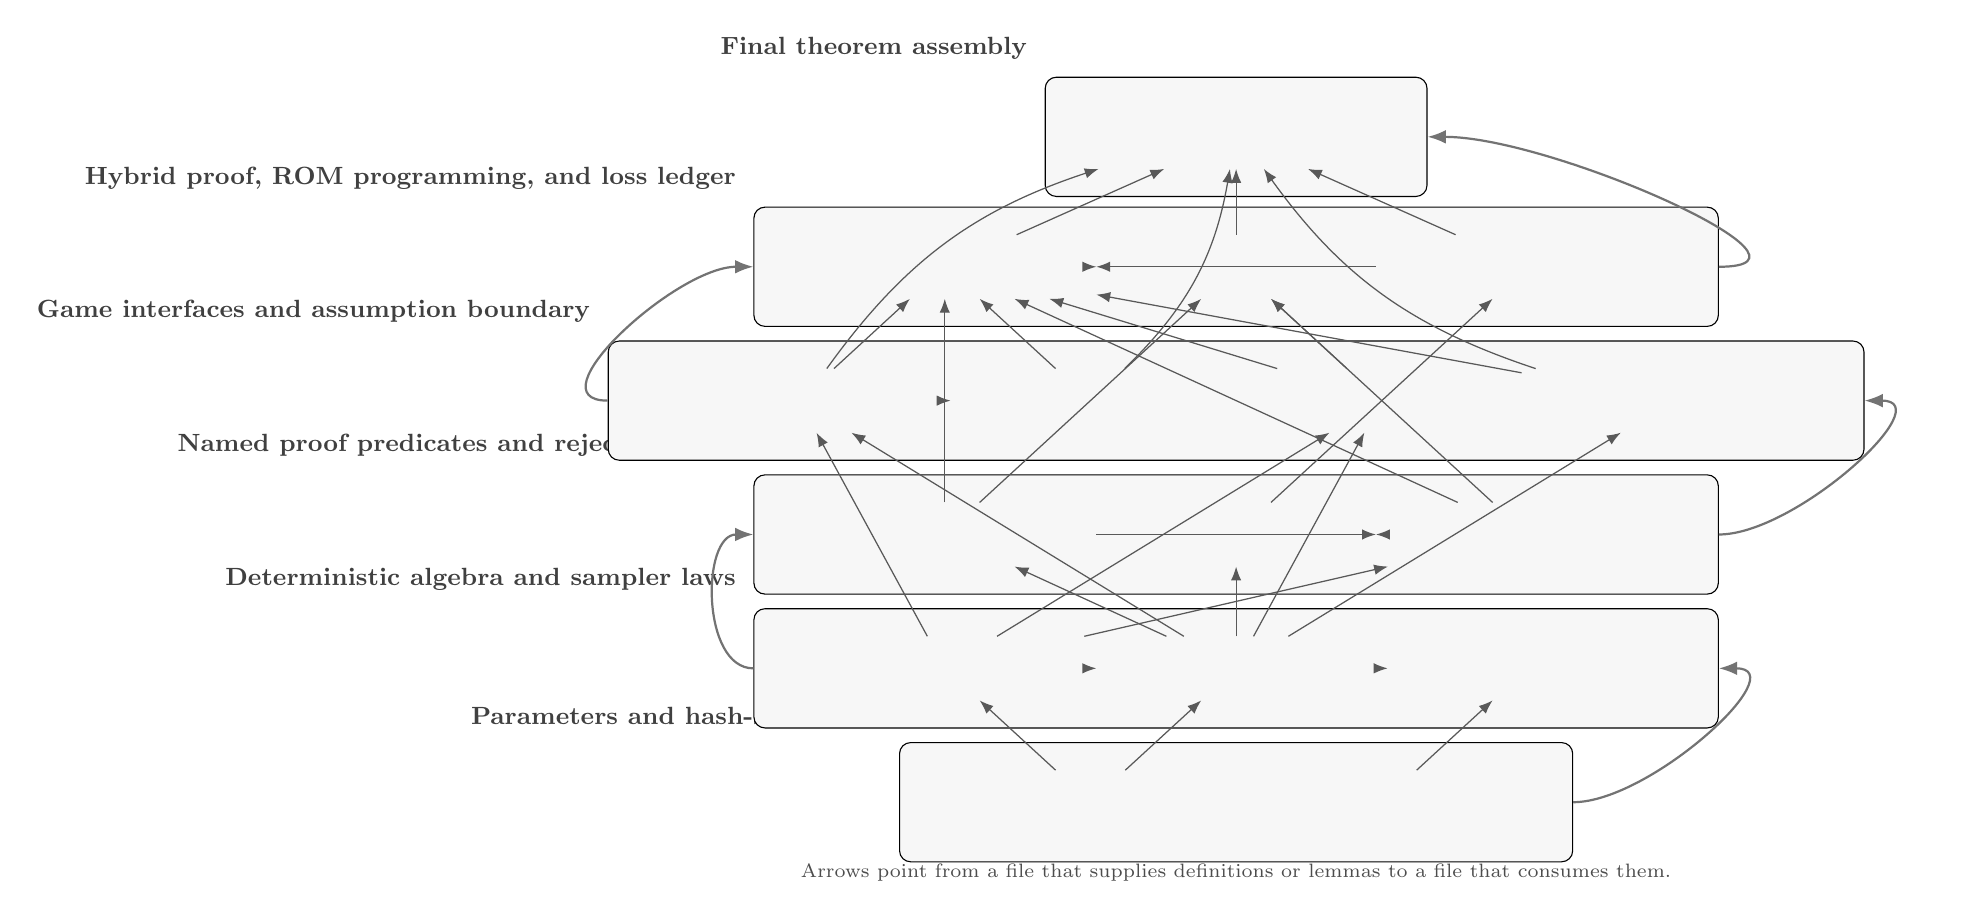
\begin{tikzpicture}[
  >=Latex,
  file/.style={
    draw,
    rounded corners=2pt,
    align=center,
    font=\tiny\ttfamily,
    minimum height=8mm,
    text width=36mm,
    fill=white
  },
  layerbox/.style={
    draw,
    rounded corners=4pt,
    fill=black!3,
    inner xsep=5mm,
    inner ysep=3.5mm
  },
  layerlabel/.style={font=\bfseries\small, text=black!75},
  flow/.style={->, line width=0.45pt, draw=black!65},
  broadflow/.style={->, line width=0.8pt, draw=black!55},
  note/.style={font=\scriptsize, align=center, text=black!70}
]

\node[file, fill=red!9] (security) at (0,9.0)
  {HAETAE\_Security.ec};

\node[file, fill=orange!12] (hop) at (-3.7,7.35)
  {HAETAE\_HopGames.ec};
\node[file, fill=orange!12] (romprog) at (0,7.35)
  {HAETAE\_ROM\_Programming.ec};
\node[file, fill=orange!12] (reductions) at (3.7,7.35)
  {HAETAE\_Reductions.ec};

\node[file, fill=yellow!14] (scheme) at (-5.55,5.65)
  {HAETAE\_Scheme.ec};
\node[file, fill=yellow!14] (sigrom) at (-1.85,5.65)
  {Sig\_ROM.ec};
\node[file, fill=yellow!14] (haetaerom) at (1.85,5.65)
  {HAETAE\_ROM.ec};
\node[file, fill=yellow!14] (assumptions) at (5.55,5.65)
  {HAETAE\_Assumptions.ec};

\node[file, fill=green!10] (transcript) at (-3.7,3.95)
  {HAETAE\_Transcript.ec};
\node[file, fill=green!10] (events) at (0,3.95)
  {HAETAE\_Events.ec};
\node[file, fill=green!10] (rejection) at (3.7,3.95)
  {HAETAE\_Rejection.ec};

\node[file, fill=blue!8] (dist) at (-3.7,2.25)
  {HAETAE\_Distributions.ec};
\node[file, fill=blue!8] (algebra) at (0,2.25)
  {HAETAE\_Algebra.ec};
\node[file, fill=blue!8] (fips) at (3.7,2.25)
  {HAETAE\_FIPS202.ec};

\node[file, fill=violet!8] (params) at (-1.85,0.55)
  {HAETAE\_Params.ec};
\node[file, fill=violet!8] (keccak) at (1.85,0.55)
  {HAETAE\_Keccak1600.ec};

\node[layerbox, fit=(params)(keccak)] (layer0) {};
\node[layerlabel, above left=1mm and 1mm of layer0.north west]
  {Parameters and hash-state base};

\node[layerbox, fit=(dist)(algebra)(fips)] (layer1) {};
\node[layerlabel, above left=1mm and 1mm of layer1.north west]
  {Deterministic algebra and sampler laws};

\node[layerbox, fit=(transcript)(events)(rejection)] (layer2) {};
\node[layerlabel, above left=1mm and 1mm of layer2.north west]
  {Named proof predicates and rejection facts};

\node[layerbox, fit=(scheme)(sigrom)(haetaerom)(assumptions)] (layer3) {};
\node[layerlabel, above left=1mm and 1mm of layer3.north west]
  {Game interfaces and assumption boundary};

\node[layerbox, fit=(hop)(romprog)(reductions)] (layer4) {};
\node[layerlabel, above left=1mm and 1mm of layer4.north west]
  {Hybrid proof, ROM programming, and loss ledger};

\node[layerbox, fit=(security)] (layer5) {};
\node[layerlabel, above left=1mm and 1mm of layer5.north west]
  {Final theorem assembly};

\draw[flow] (keccak) -- (fips);
\draw[flow] (params) -- (algebra);
\draw[flow] (params) -- (dist);
\draw[flow] (fips) -- (algebra);
\draw[flow] (algebra) -- (dist);

\draw[flow] (algebra) -- (transcript);
\draw[flow] (algebra) -- (events);
\draw[flow] (dist) -- (rejection);
\draw[flow] (transcript) -- (rejection);
\draw[flow] (events) -- (rejection);

\draw[flow] (sigrom) -- (scheme);
\draw[flow] (algebra) -- (scheme);
\draw[flow] (dist) -- (scheme);
\draw[flow] (algebra) -- (haetaerom);
\draw[flow] (dist) -- (haetaerom);
\draw[flow] (algebra) -- (assumptions);

\draw[flow] (haetaerom) -- (romprog);
\draw[flow] (transcript) -- (romprog);
\draw[flow] (rejection) -- (romprog);
\draw[flow] (events) -- (reductions);
\draw[flow] (transcript) -- (hop);
\draw[flow] (rejection) -- (hop);
\draw[flow] (scheme) -- (hop);
\draw[flow] (sigrom) -- (hop);
\draw[flow] (haetaerom) -- (hop);
\draw[flow] (assumptions) -- (hop);
\draw[flow] (romprog) -- (hop);
\draw[flow] (reductions) -- (hop);

\draw[flow] (hop) -- (security);
\draw[flow] (romprog) -- (security);
\draw[flow] (reductions) -- (security);
\draw[flow] (scheme) to[bend left=18] (security);
\draw[flow] (sigrom) to[bend right=18] (security);
\draw[flow] (assumptions) to[bend left=18] (security);

\draw[broadflow] (layer0.east) to[out=0,in=0] (layer1.east);
\draw[broadflow] (layer1.west) to[out=180,in=180] (layer2.west);
\draw[broadflow] (layer2.east) to[out=0,in=0] (layer3.east);
\draw[broadflow] (layer3.west) to[out=180,in=180] (layer4.west);
\draw[broadflow] (layer4.east) to[out=0,in=0] (layer5.east);

\node[note] at (0,-0.35)
  {Arrows point from a file that supplies definitions or lemmas to a file that consumes them.};

\end{tikzpicture}%
}
\caption{Layered structure of the active EasyCrypt files in the HAETAE provable-security proof surface.}
\label{fig:ec-file-structure}
\end{figure}


The structure is designed this way for a machine-checking reason and for a
cryptographic reason.  The machine-checking reason is that EasyCrypt proof
obligations are easier to audit when deterministic facts, probabilistic
programs, bad-event bounds, assumption games, and final real-arithmetic
composition are not mixed in the same file.  The cryptographic reason is that a
reduction proof has several trust boundaries: algebraic modeling, random-oracle
modeling, hardness assumptions, simulation failures, and final advantage
composition.  The file structure makes those boundaries visible.

\begin{longtable}{p{0.26\textwidth}p{0.28\textwidth}p{0.36\textwidth}}
\toprule
\textbf{Layer} & \textbf{Files} & \textbf{Reason for the design} \\
\midrule
\endfirsthead
\toprule
\textbf{Layer} & \textbf{Files} & \textbf{Reason for the design} \\
\midrule
\endhead
Parameters and hash-state base &
\file{HAETAE_Params.ec}, \file{HAETAE_Keccak1600.ec} &
The finite parameter vocabulary and byte/lane state vocabulary must be fixed
before algebra, sampling, or hash-shaped operations can be typed. \\
Deterministic algebra and sampler laws &
\file{HAETAE_FIPS202.ec}, \file{HAETAE_Algebra.ec},
\file{HAETAE_Distributions.ec} &
Pure algebraic equations and distribution support lemmas are reusable
mathematical facts.  Keeping them below the games prevents probabilistic proof
scripts from repeatedly unfolding deterministic definitions. \\
Named proof predicates and rejection facts &
\file{HAETAE_Transcript.ec}, \file{HAETAE_Events.ec},
\file{HAETAE_Rejection.ec} &
Transcript validity, acceptance events, and rejection predicates are shared by
ROM programming and game hopping.  Naming them once avoids inconsistent
restatements of the same bad events. \\
Game interfaces and assumption boundary &
\file{Sig_ROM.ec}, \file{HAETAE_ROM.ec}, \file{HAETAE_Scheme.ec},
\file{HAETAE_Assumptions.ec} &
The generic signature experiment, the HAETAE random-oracle domain, the concrete
scheme adapter, and the MLWE/Module-SIS games form the formal boundary between
the model and the cryptographic assumptions. \\
Hybrid proof, ROM programming, and loss ledger &
\file{HAETAE_ROM_Programming.ec}, \file{HAETAE_HopGames.ec},
\file{HAETAE_Reductions.ec} &
Stateful game hops, counted random-oracle bad events, and real-valued loss
normalization are distinct proof obligations.  Separating them makes each loss
term traceable to the lemma that introduces it. \\
Final theorem assembly &
\file{HAETAE_Security.ec} &
The public correctness and security theorem should compose already checked
facts.  This keeps the top-level theorem readable and prevents hidden new game
transformations from being introduced during final arithmetic. \\
\bottomrule
\end{longtable}

This design also explains the recommended reading order below.  A reader who
starts at the bottom sees the vocabulary and reusable lemmas first; a reader
who starts at the top sees the final theorem first and can follow each imported
obligation back to the file that proves it.

\section{Per-File Mathematical Explanation of the Proof Scripts}
\label{sec:per-file-proof-script-explanation}

This section explains why each manifest file is written in its current proof
style.  The point is not only to say what the file contains, but to explain the
mathematical reason for the local EasyCrypt script structure.

\subsection*{HAETAE\_Security.ec}

This is the theorem-assembly script.  Mathematically, it proves that the
probability of winning the HAETAE \eufcma{} experiment is bounded by a sequence
of intermediate game probabilities and then by the final concrete expression.
The script is therefore written mostly as applications of previously proved
inequalities, followed by real-arithmetic normalization.

The characteristic proof pattern is:

\begin{lstlisting}[language=EasyCrypt]
apply (ler_trans <intermediate probability expression>).
apply ler_add.
rewrite haetae_euf_bound_groupedE.
\end{lstlisting}

This style is intentional.  The file should not hide new game definitions
inside the final theorem.  It should expose exactly which hop bounds and
hardness bounds are assumed as hypotheses, combine them with transitivity of
\(\leq\), and rewrite the result into the public HAETAE bound.  After the
retirement of \file{HAETAE_GameHops.ec}, the small bridge proof that composes
the NMA, MLWE, bimodal, and Module-SIS terms is written directly here, because
it is part of the public theorem interface rather than a separate game layer.

\subsection*{Sig\_ROM.ec}

This file is written as a generic mathematical interface for signature games in
the random-oracle model.  Its types are abstract carrier sets for keys,
messages, contexts, signatures, random-oracle queries, and random-oracle
outputs.  Its modules are game functors: given a hash oracle, a scheme, and an
adversary, they construct correctness, \eufcma{}, UF-NMA, and SUF-CMA
experiments.

The most important proof script is the NMA-to-CMA adapter proof
\ec{nma_as_cma_exact}.  It is an equivalence proof because the mathematical
claim is equality of two experiments, not a loose inequality.  The CMA game
with the adapter and the NMA game execute the same adversary-facing behavior
when no signing oracle information is used.  The script uses relational
reasoning so later HAETAE files can replace an active chosen-message interface
by a passive no-message interface without reproving generic signature-game
facts.

\subsection*{HAETAE\_HopGames.ec}

This is the main hybrid-game script.  Mathematically, it expands the informal
paper proof phrase ``move through a sequence of games'' into named
probabilistic programs, invariants, bad events, and probability inequalities.
The file is long because stateful game transformations cannot be justified by
real arithmetic alone.

The script is written in stages: simulated signing, transcript logging,
ROM-internal execution, public simulation, paper simulation, rejection
simulation, exact-hyperball sampling, budgeted random-oracle programming, and
special-soundness extraction.  Equivalence proofs are used when two games have
the same result under a coupling.  Hoare proofs are used when the mathematical
claim is invariant preservation, such as transcript-log consistency, ROM query
coverage, or query-budget discipline.  Probability inequalities are used when a
bad event or sampler-freshness term accounts for the difference between two
games.  This mixed proof style mirrors the mathematics: exact couplings,
state-invariant preservation, and fundamental-lemma loss accounting are
different proof obligations and are kept syntactically distinct.

\subsection*{HAETAE\_Reductions.ec}

This file is the real-arithmetic ledger for the proof.  It defines the concrete
loss terms, hardness terms, query-budget expressions, grouped bound forms, and
non-negativity facts consumed by the top-level theorem.

The proofs are written mostly as rewriting and order reasoning because the
mathematical content is normalization of real expressions.  For example, a game
file may produce a sum in operational form, while the final theorem needs the
same loss written in the grouped form used in the dissertation.  Keeping these
lemmas here prevents the game-hop scripts from being cluttered with arithmetic
bookkeeping and prevents the top-level security theorem from depending on
ad-hoc algebraic rearrangements.

\subsection*{HAETAE\_ROM.ec}

This file gives the typed random-oracle domain used by the HAETAE model.  The
mathematical purpose is to separate message-hash queries, challenge-hash
queries, matrix-expansion queries, and sampler-expansion queries into distinct
constructors and projections.

The proof scripts are small because most claims are definitional projection and
losslessness facts.  They are nevertheless essential: later sampler-freshness
arguments need to state precisely that the only dangerous collision is with the
fresh \ec{sampler_expand_query}.  The file is written as a typed interface so
that EasyCrypt prevents accidental confusion between different hash-query
roles.

\subsection*{HAETAE\_ROM\_Programming.ec}

This file formalizes the random-oracle programming layer.  Mathematically, it
turns the fundamental-lemma argument into concrete state: programming sites,
query logs, clear events, bad events, counted events, and min-entropy events.

The script is written as a collection of preservation lemmas and probability
bounds.  Preservation lemmas show that lazy-RO operations keep the relevant
``clear'' predicates true unless a named bad event occurs.  Bound lemmas then
turn counted bad events into real loss terms.  This separation matches the
usual cryptographic proof: first prove the simulation is exact outside a bad
event, then bound the probability of the bad event.

\subsection*{HAETAE\_Scheme.ec}

This file is an adapter between the generic signature-game interface and the
HAETAE model.  Mathematically, it instantiates abstract signature-game types
with HAETAE public keys, secret keys, messages, contexts, signatures, random
oracle queries, and random oracle outputs.

The script is deliberately thin.  It defines the \ec{HAETAE} scheme module so
the generic games in \file{Sig_ROM.ec} can execute \ec{kg}, \ec{sign}, and
\ec{verify}.  It does not try to prove the full security theorem locally,
because that would mix interface alignment with algebra, rejection sampling,
ROM programming, and game hopping.  Its value is making the later proof scripts
operate over one uniform scheme object.

\subsection*{HAETAE\_Transcript.ec}

This file explains how a signature execution is represented as a mathematical
transcript.  The transcript records the public key, message, context,
commitment data, challenge, response, hint, token, rejection branch, and
validity predicates needed by the reduction.

The proof scripts are mainly definitional decomposition and implication lemmas.
They are written this way because later reductions need small, named facts such
as ``a valid transcript exposes the challenge query'' or ``a valid forking pair
gives the public algebraic equations.''  Without this file, the hop games would
need to repeatedly unfold large transcript predicates.  With it, the proof can
move from a winning signature event to the algebraic objects required for
bimodal self-target and Module-SIS reductions.

\subsection*{HAETAE\_Events.ec}

This file names the basic rejection and acceptance events.  Mathematically, it
packages predicates such as key-generation rejection failure, signing rejection
failure, verification rejection failure, and accepted-transcript
rejection-freeness.

The scripts are intentionally short and mostly definitional.  Their purpose is
not to perform a deep reduction, but to give the game-hop files stable event
names.  This is why the file contains small lemmas showing that the current
model satisfies the event predicates.  The design keeps later proofs readable:
they refer to named events instead of re-expanding the low-level rejection and
verification definitions at every hop.

\subsection*{HAETAE\_Assumptions.ec}

This file defines the abstract hardness games and reduction interfaces.  The
mathematical role is to state where the machine-checked game proof stops and
where cryptographic hardness assumptions begin.

The script is written with module types, game modules, and relation predicates
rather than unchecked theorem axioms.  This matters for trust accounting:
EasyCrypt checks that the final theorem refers to explicit MLWE, Module-SIS,
and bimodal self-target game probabilities.  The file therefore makes the
assumptions visible as formal game interfaces.  It does not prove those
hardness assumptions, and the rest of the proof must consume them as advantage
terms.

\subsection*{HAETAE\_Distributions.ec}

This file supplies the probability laws used by the scheme and the game hops.
Mathematically, it defines distributions for bytes, seeds, CRHs, signing
randomness, coefficients, polynomial vectors, matrices, challenges, bounded
samples, and exact-hyperball samples.

The proof scripts are written around losslessness, support, domain, and
point-probability lemmas.  These are the facts that make later probability
bounds legal.  For example, sampler-freshness arguments require a support-size
or point-bound statement; rejection-sampling arguments require domain and
well-formedness statements.  The file isolates those distribution facts so the
game-hop proof can cite them rather than redoing measure-theoretic reasoning at
each call site.

\subsection*{HAETAE\_Rejection.ec}

This file formalizes the rejection-sampling side of the proof.  Mathematically,
it connects signing samples, rejection predicates, accepted-signature
conditions, and rejection loss terms.

The script separates deterministic predicate implications from probabilistic
loss accounting.  Deterministic lemmas show that accepted samples satisfy the
well-formedness and event predicates needed by transcript and verification
arguments.  Probability lemmas relate the rejection process to the loss terms
used by the final theorem.  This organization is necessary because rejection
sampling is both an algebraic validity condition and a probabilistic source of
loss.

\subsection*{HAETAE\_Algebra.ec}

This is the deterministic mathematical foundation of the model.  It defines the
carrier types and operations for bytes, seeds, polynomials, vectors, matrices,
keys, signatures, commitments, challenges, and the verification equations.

The proof scripts are mostly rewriting, list reasoning, range reasoning, and
algebraic simplification.  They are kept separate from probabilistic games
because these facts are pure mathematics over the modeled carrier sets.  The
later proof should be able to cite a named algebra lemma without unfolding the
definition of polynomial-vector arithmetic or commitment reconstruction inside
a game equivalence proof.

\subsection*{HAETAE\_Params.ec}

This file records the parameter modes and constants.  Mathematically, it fixes
the finite set of HAETAE modes and exposes functions such as dimensions,
byte-lengths, and bounds as mode-indexed constants.

The proof script is simple because the file's job is to make parameter facts
available to the type checker and arithmetic lemmas.  It is written as
definitions and basic positivity/range facts rather than as a cryptographic
proof.  The later algebra, distribution, rejection, and reduction files depend
on these constants being explicit and reusable.

\subsection*{HAETAE\_FIPS202.ec}

This file gives the modeled FIPS202/SHAKE support used by the formal HAETAE
model.  Mathematically, it supplies deterministic hash-interface functions and
size/rate/capacity facts needed by the typed model.

The script is not a standard-model security proof for SHAKE.  It is written as
deterministic interface support: operations define modeled hash behavior, and
lemmas establish the simple structural facts later files need.  This separation
keeps the final theorem honest: the checked security theorem remains a
random-oracle-model theorem, even though the model includes FIPS202-flavored
support definitions.

\subsection*{HAETAE\_Keccak1600.ec}

This file supplies the low-level Keccak state vocabulary used by the modeled
hash support.  Mathematically, it is a deterministic bit/byte and lane/state
model rather than a game-based security proof.

The proof scripts establish range, indexing, state-shape, and round-function
facts by unfolding definitions and reasoning about finite lists and integers.
It is written separately from \file{HAETAE_FIPS202.ec} so the byte-level and
state-level mechanics do not obscure the higher-level FIPS202 interface.  The
provable-security theorem uses this layer only as modeled hash support; it does
not derive random-oracle security from Keccak.

\section{Recommended Reading Order}

The proof is easiest to follow from the bottom of the dependency graph upward:

\begin{enumerate}[leftmargin=*]
  \item Read \file{HAETAE_Params.ec}, \file{HAETAE_Keccak1600.ec}, and
  \file{HAETAE_FIPS202.ec} to understand the parameter and hash vocabulary.
  \item Read \file{HAETAE_Algebra.ec} and \file{HAETAE_Distributions.ec} to see
  the mathematical carrier sets, operations, and sampler laws.
  \item Read \file{Sig_ROM.ec}, \file{HAETAE_ROM.ec}, and
  \file{HAETAE_Scheme.ec} to understand the generic signature experiment and
  the HAETAE instantiation.
  \item Read \file{HAETAE_Transcript.ec}, \file{HAETAE_Events.ec}, and
  \file{HAETAE_Rejection.ec} to see how signing, verification, rejection, and
  transcript validity become named predicates.
  \item Read \file{HAETAE_ROM_Programming.ec} to understand the counted
  random-oracle programming events and losses.
  \item Read \file{HAETAE_HopGames.ec} to follow the detailed game hops.
  \item Read \file{HAETAE_Reductions.ec} to see how the loss terms are grouped.
  \item Read \file{HAETAE_Security.ec} last.  It assembles the earlier lemmas
  into externally usable correctness and security statements.
\end{enumerate}

\section{How to Follow the Top-Level Theorem}

Start in \file{HAETAE_Security.ec}.  The opening imports show the complete
direct dependency surface:

\begin{lstlisting}[language=EasyCrypt]
require import Sig_ROM HAETAE_Scheme HAETAE_Algebra HAETAE_Distributions.
require import HAETAE_Reductions HAETAE_Assumptions.
require import HAETAE_Rejection.
require import HAETAE_Transcript HAETAE_ROM_Programming.
require import HAETAE_HopGames.
\end{lstlisting}

The proof has two main families.

\begin{description}
  \item[Correctness.]
  The \ec{correctness_obligation} definition records the required relationship
  between key generation, signing, and verification.  The lemmas
  \ec{correctness_obligation_holds} and \ec{correctness_perfect} connect that
  obligation to the generic correctness experiment.

  \item[Security.]
  The \ec{euf_cma_security} family composes a Fiat-Shamir-with-aborts hop, a
  no-message attack boundary, MLWE and Module-SIS hardness terms, bimodal
  self-target-to-MSIS reduction loss, and random-oracle programming losses.
\end{description}

When reading a top-level lemma, separate the hypotheses into three groups:

\begin{enumerate}[leftmargin=*]
  \item A game-hop hypothesis comparing two EasyCrypt experiments.
  \item A reduction or hardness-game hypothesis bounding an intermediate game.
  \item Arithmetic facts from \file{HAETAE_Reductions.ec} that normalize the
  concrete loss expression.
\end{enumerate}

This discipline prevents a common mistake: the theorem does not assert that
MLWE or Module-SIS is unconditionally hard.  It composes the checked game proof
with abstract hardness-game advantages.

\section{How to Follow the Main Hop File}

\file{HAETAE_HopGames.ec} is the main body of the machine-checked hybrid proof.
Do not try to read it linearly on the first pass.  Instead, search for the
modules and lemma families that correspond to the paper proof stages:

\begin{lstlisting}[language=bash]
rg -n "module .*EUF|module .*NMA|lemma .*hop|lemma .*lifting" \
  provable-security/easycrypt/HAETAE_HopGames.ec
\end{lstlisting}

The important stages are:

\begin{enumerate}[leftmargin=*]
  \item Real signing is related to simulated signing.
  \item Simulated signing is related to transcript-based games.
  \item Transcript games are related to ROM-internal games.
  \item Clean-event and bad-event predicates isolate the failure cases.
  \item Budgeted wrappers count adversary hash calls and signing calls.
  \item Sampler freshness bounds the probability that a fresh sampler query was
  already asked by the adversary.
  \item Exact-hyperball and rejection-sampling games connect the simulated
  transcript proof to the algebraic hardness reductions.
\end{enumerate}

For each hop lemma, identify:

\begin{itemize}[leftmargin=*]
  \item the two experiments whose probabilities are compared;
  \item the bad event or loss term that accounts for the difference;
  \item the invariant preserved by the corresponding Hoare or equivalence proof;
  \item the later top-level lemma that consumes the hop.
\end{itemize}

\section{Checking the Manifest Against the Directory}

To check that the root-level active \file{.ec} files match the manifest:

\begin{lstlisting}[language=bash]
find . -maxdepth 1 -name '*.ec' -printf '%f\n' | sort
sed -n '/^[^#[:space:]]/p' provable-security/proof-files.txt | sort
\end{lstlisting}

At the time of this guide, both commands should list the same sixteen proof
files.  Additional historical or validation files belong under \file{rubbish/}
unless they are intentionally reintroduced into the manifest and verified.

\section{Regenerating the Dissertation Inventory}

The dissertation records an inventory of the checked surface.  After changing
the manifest, regenerate the count file:

\begin{lstlisting}[language=bash]
make -C dissertation inventory
\end{lstlisting}

The current inventory total is:

\begin{lstlisting}
TOTAL,22046,63,678,113,1088,0,105
\end{lstlisting}

The columns are:

\begin{lstlisting}
file,lines,types,ops,modules,lemmas,axioms,hoare_equiv
\end{lstlisting}

The important trust-boundary fact is the axiom count.  A zero manifest-local
axiom count means the final theorem is not installed by an unchecked
\ec{axiom}.  It does not remove the cryptographic assumptions; those assumptions
are modeled as abstract games, hardness terms, modules, and parameters.

\section{Building the Dissertation}

The dissertation is separate from the proof gate.  It documents the checked
artifact but is not itself the EasyCrypt proof kernel.

Build it with:

\begin{lstlisting}[language=bash]
make -C dissertation
\end{lstlisting}

The expected output is:

\begin{lstlisting}[language=bash]
dissertation/main.pdf
\end{lstlisting}

After a build, check for serious LaTeX problems:

\begin{lstlisting}[language=bash]
rg -n "(^!|Fatal|Emergency|undefined|Undefined|Rerun|Label\\(s\\))" \
  dissertation/main.log
\end{lstlisting}

Overfull boxes and font-shape warnings are formatting issues, not proof
failures.  Undefined references, fatal errors, and failed PDF generation should
be fixed before using the dissertation as documentation for the proof state.

\section{Changing the Proof Safely}

Use this sequence for any proof-surface change:

\begin{enumerate}[leftmargin=*]
  \item Run \file{sh provable-security/verify-provable-security.sh} first and
  save the baseline result.
  \item Edit the root file and the corresponding
  \file{provable-security/easycrypt/} copy, or deliberately explain why only
  one copy changes.
  \item Compile the directly edited file first.  For example:
\begin{lstlisting}[language=bash]
easycrypt compile provable-security/easycrypt/HAETAE_Security.ec \
  -max-provers 1 \
  -I provable-security/easycrypt \
  -I kyber-security
\end{lstlisting}
  \item Run the full proof gate.
  \item If the manifest changed, update dissertation manifest tables and run:
\begin{lstlisting}[language=bash]
make -C dissertation inventory
make -C dissertation
\end{lstlisting}
  \item Search for stale references to removed files or theorem names:
\begin{lstlisting}[language=bash]
rg -n "RemovedFileName|RemovedLemmaName" .
\end{lstlisting}
\end{enumerate}

\section{Interpreting Failure Modes}

\begin{longtable}{p{0.32\textwidth}p{0.58\textwidth}}
\toprule
\textbf{Symptom} & \textbf{Likely cause and first action} \\
\midrule
\endfirsthead
\toprule
\textbf{Symptom} & \textbf{Likely cause and first action} \\
\midrule
\endhead
Missing manifest file &
The manifest lists a file that is missing from the copied proof surface.  Either
restore the file or remove it from the manifest only if it is genuinely outside
the checked proof. \\
Unknown theory or identifier &
An import was removed, a file was moved, or a theorem was renamed.  Search for
the missing name and check the direct imports of the failing file. \\
Probability inequality proof fails &
The game-hop statement or concrete loss expression changed.  Check the relevant
lemma in \file{HAETAE_Reductions.ec} before changing top-level arithmetic. \\
Hoare or equivalence proof fails &
A game procedure or invariant changed.  Re-read the precondition, postcondition,
and modified procedure body before editing tactics. \\
Manifest passes but dissertation is stale &
The machine-checked proof is still valid, but documentation is out of sync.
Regenerate counts and update manifest/dependency tables. \\
\bottomrule
\end{longtable}

\section{What Is Outside the Verified Claim}

The following are not established by the central EasyCrypt proof gate:

\begin{itemize}[leftmargin=*]
  \item concrete MLWE or Module-SIS hardness estimates;
  \item a standard-model proof replacing the random oracle by SHAKE;
  \item implementation-level parsing, serialization, or constant-time behavior;
  \item a checked equivalence between every line of the HAETAE specification PDF
  and every operation in the EasyCrypt model;
  \item generated known-answer-test artifacts archived under \file{rubbish/}.
\end{itemize}

These exclusions are not defects in the proof.  They are the trust boundary that
keeps the machine-checked theorem precise.

\section{Line-by-Line Companion Guides}

The directory \file{guide/line-by-line/} contains one mathematical companion
document for each EasyCrypt file in \file{provable-security/proof-files.txt}.
Each companion preserves the source line number, the EasyCrypt line, and a
short mathematical explanation of the declaration, game step, Hoare/equivalence
claim, or proof tactic appearing on that line.  Start with
\file{guide/line-by-line/index.pdf} for the file order, then open the matching
\file{*-line-by-line-guide.pdf} for the file being read.

For a declaration-oriented view, use
\file{guide/haetae-symbolic-correspondence-guide.pdf}.  It lists every checked
\ec{type}, \ec{op}, \ec{lemma}, \ec{equiv}, and explicit \ec{hoare.} step with
the corresponding mathematical reading, such as carrier sets, total functions,
predicates, probability bounds, relational judgments, and Hoare triples.

For a narrative mathematical view, use
\file{guide/haetae-mathematical-cryptology-guide.pdf}.  It starts with a
continuous mathematical overview of the theorem statement, security games,
assumptions, game-hop chain, transcript extraction, random-oracle programming,
algebraic model, and rejection-sampling losses, then adds one chapter per
checked \file{.ec} file with a generated textbook inventory of the exact
definitions, games, lemmas, equivalence theorems, and program-logic judgments
in that file.

Regenerate the companions after changing the manifest or any checked
EasyCrypt file:

\begin{lstlisting}[language=bash]
python3 guide/generate-line-by-line-guides.py
python3 guide/generate-symbolic-correspondence-guide.py
python3 guide/generate-mathematical-chapter-details.py
make -C guide/line-by-line all
\end{lstlisting}

\section{Minimal Reproducibility Checklist}

A complete local verification pass consists of:

\begin{enumerate}[leftmargin=*]
  \item \file{easycrypt --version} succeeds.
  \item \file{sh provable-security/verify-provable-security.sh} ends with
  \ec{RESULT: PASS}.
  \item \file{provable-security/proof-files.txt} contains only intended proof
  files.
  \item No active proof file imports a file from \file{rubbish/}.
  \item If documentation was changed, \file{make -C dissertation} produces
  \file{dissertation/main.pdf}.
\end{enumerate}

After these checks, the reader has reproduced the machine-checked
provable-security verification path from the beginning: tool availability,
manifest selection, per-file EasyCrypt compilation, log inspection, and
documentation synchronization.

\end{document}
